\documentclass{../template/myrpt}
\ExamName{分光计的调整与使用}

\usepackage{multirow}
\pgfplotsset{compat=1.18}
\usetikzlibrary{arrows.meta,calc,angles,quotes,decorations.pathreplacing}
\newcolumntype{Y}{>{\centering\arraybackslash}X}
\newcolumntype{C}[1]{>{\centering\arraybackslash}m{#1}}
\newcommand{\blankcell}{\rule{0pt}{0.46cm}}

\begin{document}
\insertCoverPage

\section{实验目的}
\begin{enumerate}[label=\arabic*. ]
  \item 了解分光计的结构、作用与工作原理；
  \item 学会分光计的调整与使用方法；
  \item 了解光栅特性，并用光栅衍射测量光波波长、光栅常数、角色散和分辨本领。
\end{enumerate}

\section{实验仪器}

JJY1 型分光计、平面反射镜、低压汞灯、平面透射光栅。

\begin{figure}[htbp]
  \centering
  \begin{minipage}[t]{0.58\linewidth}
    \centering
    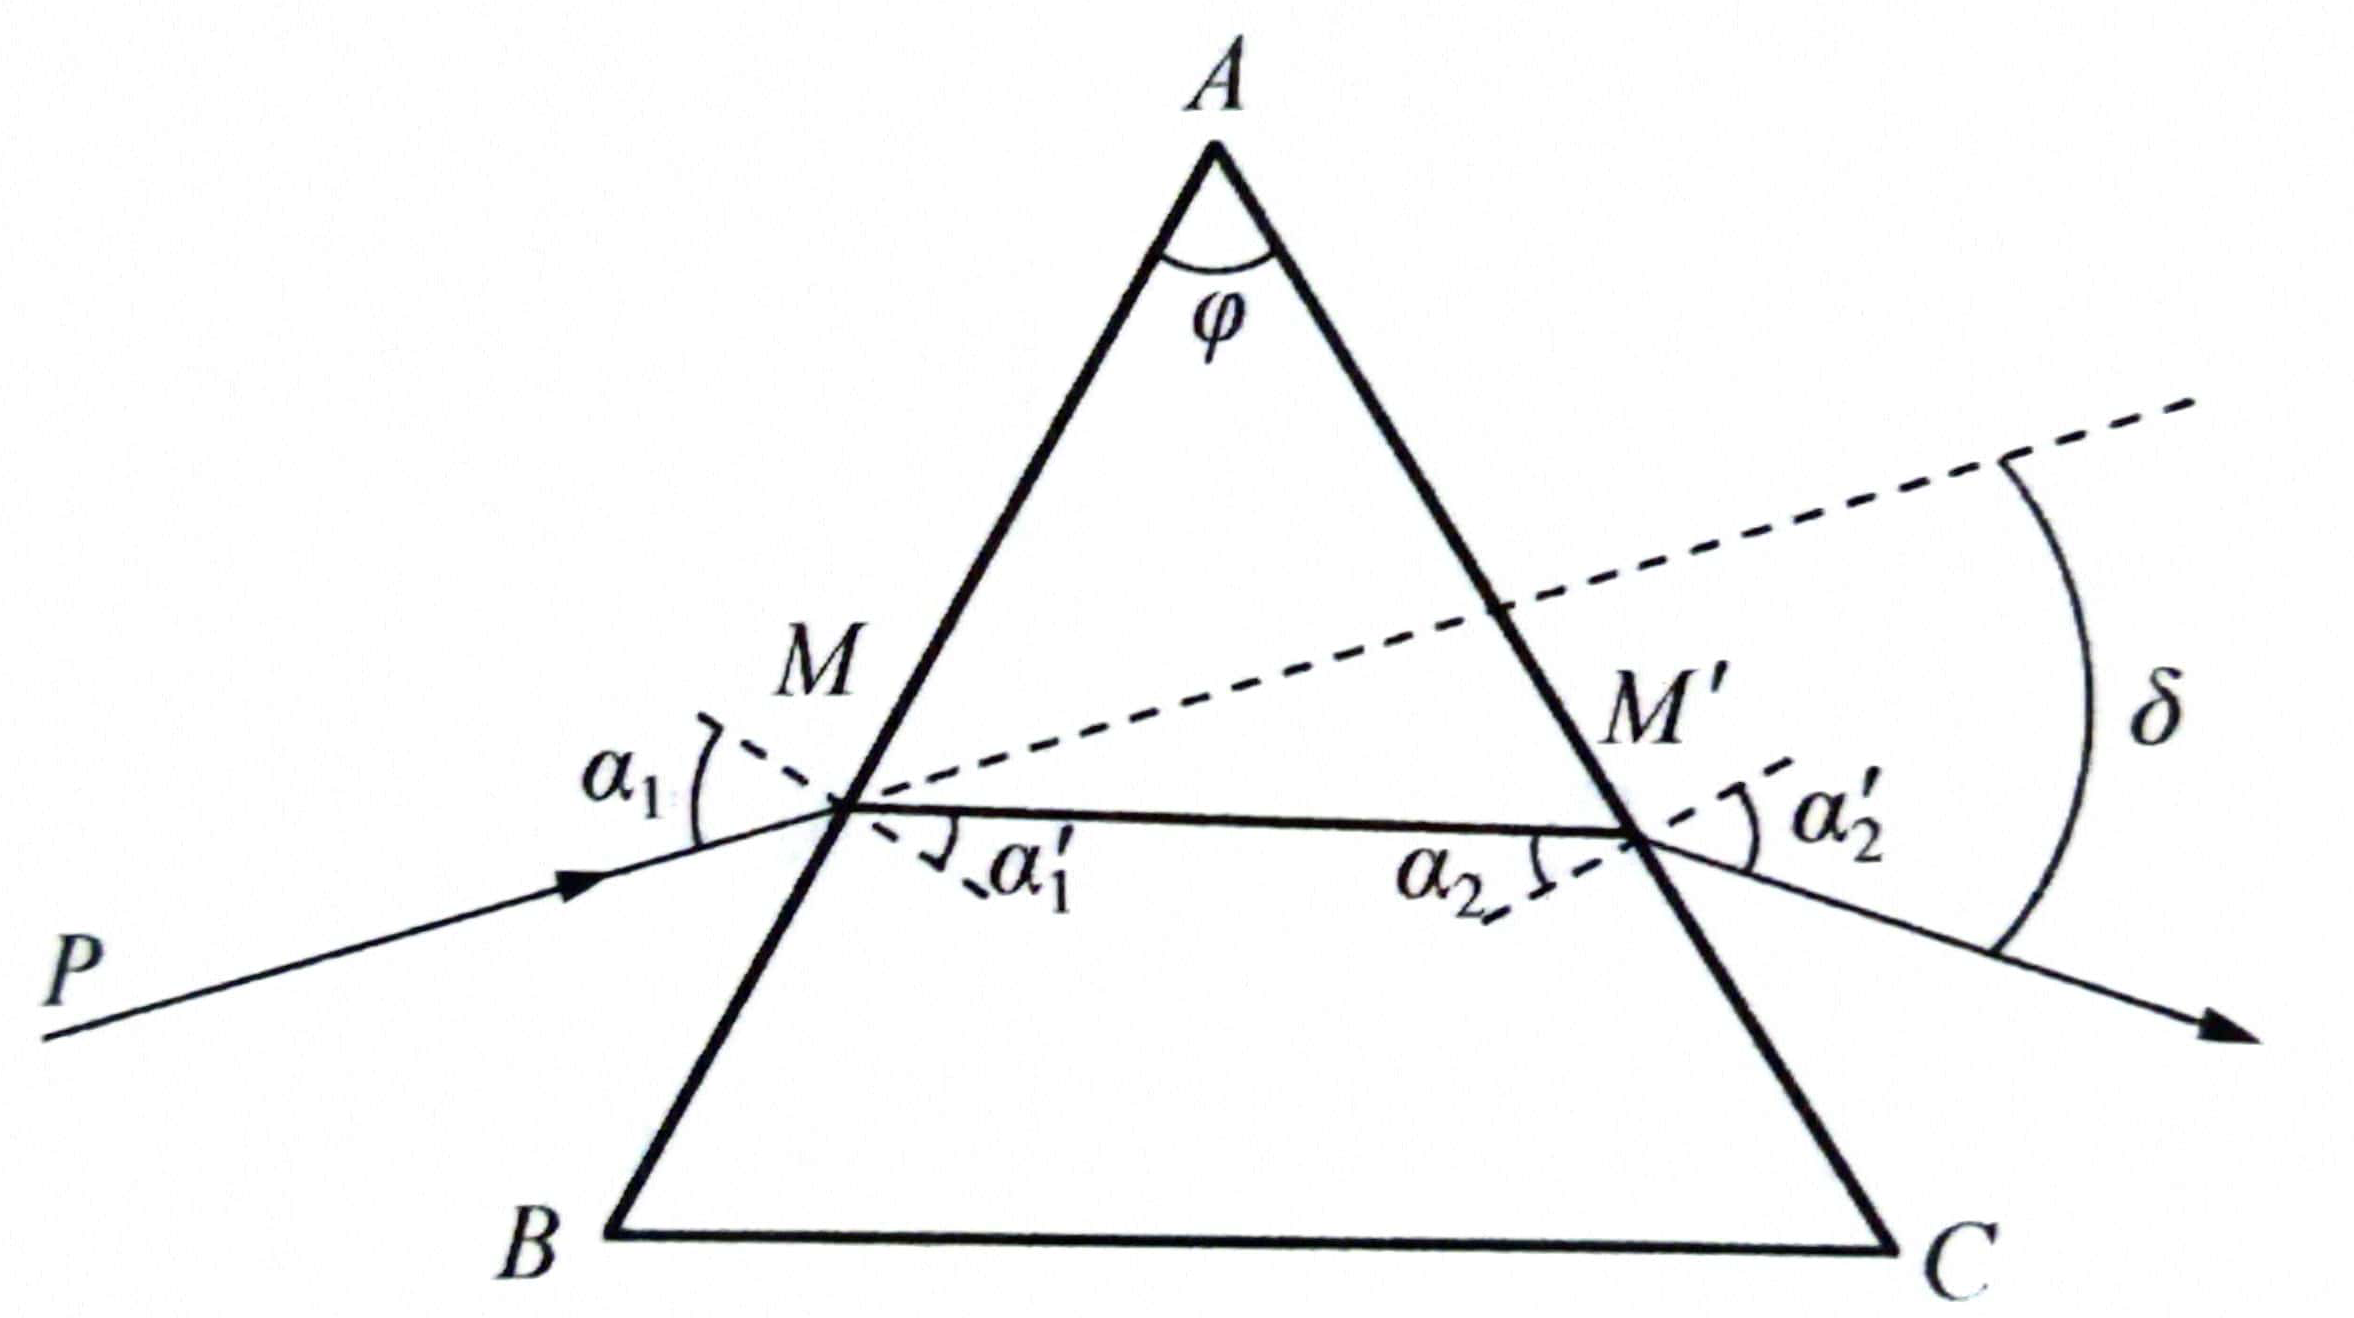
\includegraphics[width=\linewidth]{assets/apparatus.png}
    \caption{JJY1 型分光计}
    \label{fig:apparatus}
  \end{minipage}
  \hfill
  \begin{minipage}[t]{0.38\linewidth}
    \centering
    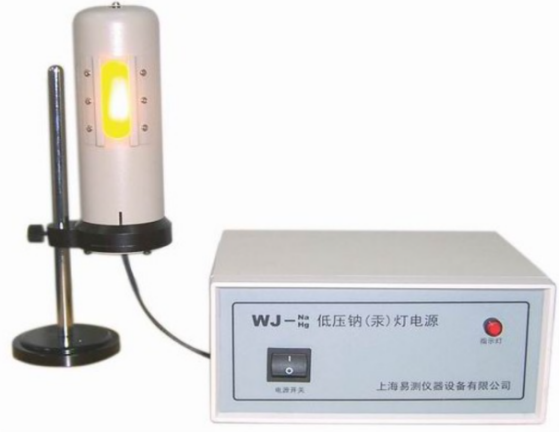
\includegraphics[width=\linewidth]{assets/apparatus-grating.png}
    \caption{分光计与低压汞灯}
    \label{fig:apparatus-grating}
  \end{minipage}
\end{figure}

\section{实验原理}

\subsection{分光计的构造与测角原理}

分光计又称分光测角仪，用于精确测量光线的偏转角。通过角度测量可以进一步得到光波波长、色散率和光栅常数等物理量。仪器主要由平行光管、载物台、望远镜和读数装置组成，结构如图~\ref{fig:spectrometer-structure} 所示。

\begin{figure}[htbp]
  \centering
  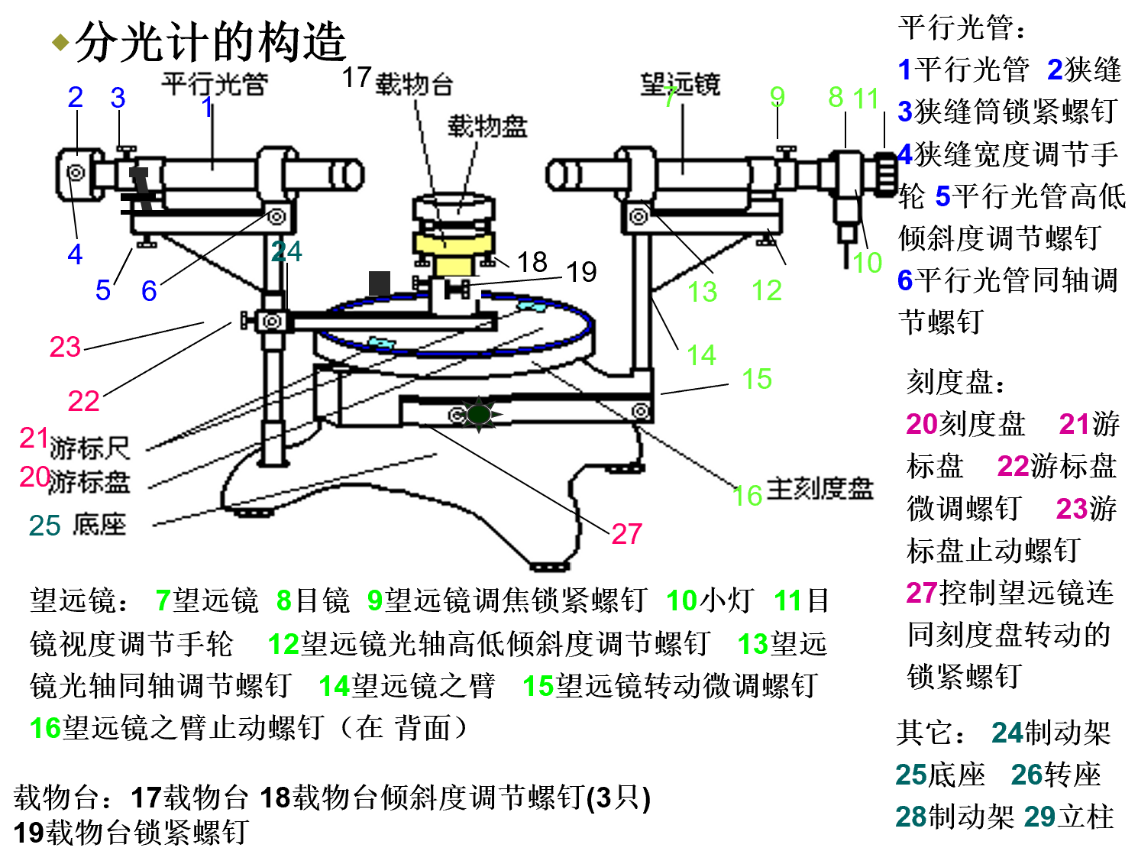
\includegraphics[width=0.78\linewidth]{assets/spectrometer-structure.png}
  \caption{分光计的主要结构}
  \label{fig:spectrometer-structure}
\end{figure}

测量两束平行光之间的夹角，实际上就是测定它们的方位角。平行光束 1、2 在望远镜焦平面上分别会聚为 $A$、$B$ 两点。焦平面上的每一点都与一定方向的平行光相对应。若望远镜光轴由平行于光束 1 转到平行于光束 2，则光轴转过的角度就是这两束光的夹角 $\theta$。

分光计度盘上有相隔约 $180^\circ$ 的两个游标窗口。设游标 I 上两束光的读数为 $\theta_1$、$\theta_2$，游标 II 上为 $\theta_1'$、$\theta_2'$，则单窗口给出
\begin{equation}
  \label{eq:angle-one}
  \theta=\lvert\theta_2-\theta_1\rvert.
\end{equation}
为消除度盘偏心差，取两窗口夹角的平均
\begin{equation}
  \label{eq:angle-mean}
  \theta=\frac{1}{2}\left(\lvert\theta_2-\theta_1\rvert+\lvert\theta_2'-\theta_1'\rvert\right).
\end{equation}
若某对读数跨越 $0^\circ/360^\circ$，应先将角度换算到同一周期后再相减。读数关系如表~\ref{table:angle-mean} 所示。

\begin{table}[htbp]
  \centering
  \caption{双游标测角}
  \label{table:angle-mean}
  \renewcommand{\arraystretch}{1.15}
  \begin{tabular}{cccc}
    \toprule
    游标 & 光线 1 & 光线 2 & 夹角 \\
    \midrule
    I & $\theta_1$ & $\theta_2$ & $\lvert\theta_2-\theta_1\rvert$ \\
    II & $\theta_1'$ & $\theta_2'$ & $\lvert\theta_2'-\theta_1'\rvert$ \\
    平均 & & & $\frac{1}{2}(\lvert\theta_2-\theta_1\rvert+\lvert\theta_2'-\theta_1'\rvert)$ \\
    \bottomrule
  \end{tabular}
\end{table}

\subsection{光栅常数和光栅方程}

衍射光栅由大量等宽、等间距、平行排列的狭缝构成。设透光缝宽为 $a$，相邻不透光部分宽度为 $b$，则光栅常数
\begin{equation}
  \label{eq:grating-constant}
  d=a+b.
\end{equation}
单位长度内的刻线数 $N=1/d$。用于可见光区的光栅每毫米可达数百到上千条。本实验使用平面透射光栅，如图~\ref{fig:grating} 所示。

\begin{figure}[!htbp]
  \centering
  % 原引用图：assets/grating.png
  % TikZ 复刻。原图：assets/grating.png
% 回退：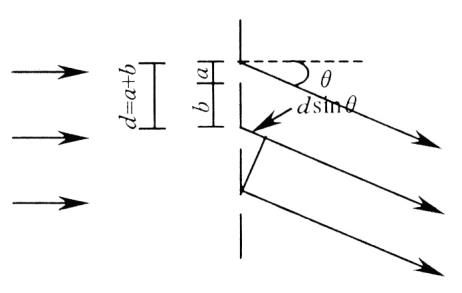
\includegraphics[width=0.62\linewidth]{assets/grating.png}
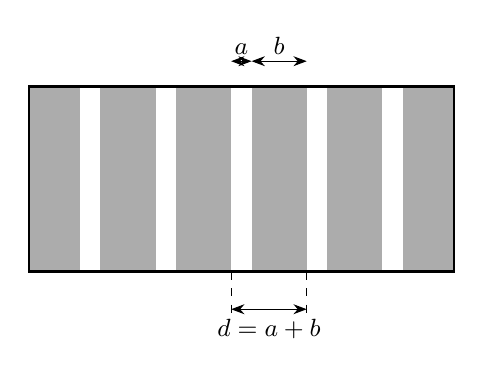
\begin{tikzpicture}[>=Stealth, font=\small]
  \def\W{5.4}
  \def\H{2.35}
  \def\slit{0.26}
  \def\barw{0.70}
  \fill[gray!65] (-\W/2,-\H/2) rectangle (\W/2,\H/2);
  \draw[thick] (-\W/2,-\H/2) rectangle (\W/2,\H/2);
  \foreach \k in {-2,-1,0,1,2} {
    \pgfmathsetmacro{\cx}{\k*(\slit+\barw)}
    \fill[white] (\cx-\slit/2,-\H/2+0.015) rectangle (\cx+\slit/2,\H/2-0.015);
  }
  \draw[<->] (-\slit/2,\H/2+0.32) -- (\slit/2,\H/2+0.32);
  \node[above=-1pt] at (0,\H/2+0.32) {$a$};
  \draw[<->] (\slit/2,\H/2+0.32) -- (\slit/2+\barw,\H/2+0.32);
  \node[above=-1pt] at ({\slit/2+\barw/2},\H/2+0.32) {$b$};
  \draw[dashed] (-\slit/2,-\H/2) -- (-\slit/2,-\H/2-0.58);
  \draw[dashed] (\slit/2+\barw,-\H/2) -- (\slit/2+\barw,-\H/2-0.58);
  \draw[<->] (-\slit/2,-\H/2-0.48) -- (\slit/2+\barw,-\H/2-0.48);
  \node[below] at ({(\barw)/2},-\H/2-0.48) {$d=a+b$};
\end{tikzpicture}

  \caption{平面透射光栅}
  \label{fig:grating}
\end{figure}

根据夫琅和费衍射理论，波长为 $\lambda$ 的平行光垂直入射光栅时，各缝衍射光在叠加处发生多光束干涉。相邻缝沿衍射角 $\varphi$ 方向的光程差为 $d\sin\varphi$，如图~\ref{fig:grating-diffraction} 所示。当
\begin{equation}
  \label{eq:grating-equation}
  d\sin\varphi=k\lambda,\qquad k=0,\pm1,\pm2,\ldots
\end{equation}
时出现干涉主极大。式~\eqref{eq:grating-equation} 称为光栅方程，$k$ 为衍射级次，$\varphi$ 为衍射光与光栅法线的夹角。

\begin{figure}[!htbp]
  \centering
  % 原引用图：assets/grating-diffraction.png
  % TikZ 复刻。原图：assets/grating-diffraction.png
% 回退：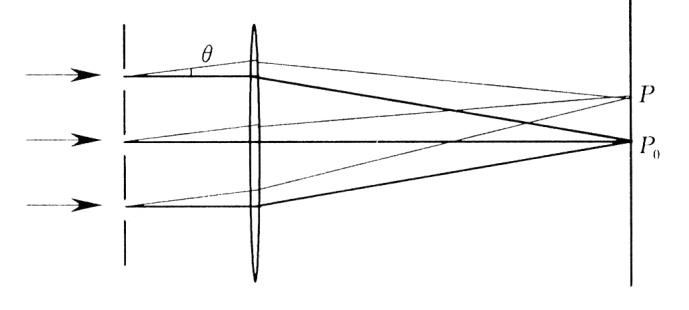
\includegraphics[width=0.88\linewidth]{assets/grating-diffraction.png}
\begin{tikzpicture}[>=Stealth, font=\small]
  \foreach \y in {-1.65,-1.43,...,1.65} {
    \filldraw[fill=gray!70, thick] (-0.08,\y-0.07) rectangle (0.08,\y+0.07);
  }
  \node[above] at (0,1.85) {光栅};
  \foreach \y in {-0.7,-0.23,0.23,0.7} {
    \draw[->, thick] (-3.0,\y) -- (-0.12,\y);
  }
  \node at (-2.1,1.15) {入射光};
  \draw[dashed] (0,-2.05) -- (0,2.05);
  \node[below left] at (0,-1.95) {法线};
  % thin biconvex lens: two shallow arcs, ends do not cross
  \draw[thick] (3.62,-1.55) .. controls (3.80,0) .. (3.62,1.55);
  \draw[thick] (3.88,-1.55) .. controls (3.70,0) .. (3.88,1.55);
  \draw[thick] (3.62,-1.55) -- (3.88,-1.55);
  \draw[thick] (3.62,1.55) -- (3.88,1.55);
  \coordinate (P0) at (7.25,0);
  \coordinate (P) at (7.25,1.12);
  \coordinate (Pp) at (7.25,-1.12);
  \draw[dashed] (0,0) -- (P0);
  \foreach \y in {-0.26,0,0.26} {
    \draw (0.10,\y) -- (3.62,\y) -- (P0);
  }
  \foreach \y in {-0.14,0,0.14} {
    \draw (0.10,\y) -- (3.62,0.72+\y) -- (P);
    \draw (0.10,\y) -- (3.62,-0.72+\y) -- (Pp);
  }
  \fill (P0) circle (1.2pt);
  \fill (P) circle (1.2pt);
  \fill (Pp) circle (1.2pt);
  \node[right] at (P0) {$P_0$ 零级};
  \node[right] at (P) {$P$ $+1$级};
  \node[right] at (Pp) {$P'$ $-1$级};
  % phi 画在光栅右侧、透镜之前，角边落在 +1 级光线上
  \coordinate (O) at (0,0);
  \coordinate (AxR) at (2.95,0);
  \coordinate (RayR) at (2.90,0.58);
  \pic[draw, angle radius=21mm, angle eccentricity=1.22,
       pic text=$\varphi$, pic text options={above}] {angle=AxR--O--RayR};
\end{tikzpicture}

  \caption{光栅衍射示意图}
  \label{fig:grating-diffraction}
\end{figure}

$\varphi=0$ 对应中央主极大。实际光栅缝数很多、缝宽很小，当光源为细长狭缝时，衍射图样是一组细锐亮线，即狭缝本身的衍射干涉条纹。

若左右两侧同级谱线的窗口读数分别为 $\theta_{\mathrm{R}}$、$\theta_{\mathrm{R}}'$ 和 $\theta_{\mathrm{L}}$、$\theta_{\mathrm{L}}'$，则衍射角
\begin{equation}
  \label{eq:diffraction-angle}
  \varphi=\frac{1}{4}\left(\lvert\theta_{\mathrm{R}}-\theta_{\mathrm{L}}\rvert+\lvert\theta_{\mathrm{R}}'-\theta_{\mathrm{L}}'\rvert\right).
\end{equation}
已知 $d$ 和 $k$ 后可由式~\eqref{eq:grating-equation} 求 $\lambda$；已知 $\lambda$ 和 $k$ 则可求 $d$。

\subsection{光栅光谱}

当入射光为复色光时，只有 $k=0$ 时各种波长的中央主极大重合，在焦平面上形成明亮的零级亮线。对其他级次，不同波长的主极大彼此分开，按短波到长波的次序在零级两侧对称排列，形成光栅光谱。$k=\pm1$ 为一级光谱，$k=\pm2$ 为二级光谱。低压汞灯的衍射光谱示意如图~\ref{fig:mercury-spectrum}。

\begin{figure}[!htbp]
  \centering
  % 原引用图：assets/mercury-spectrum.png
  % TikZ 复刻。原图：assets/mercury-spectrum.png
% 回退：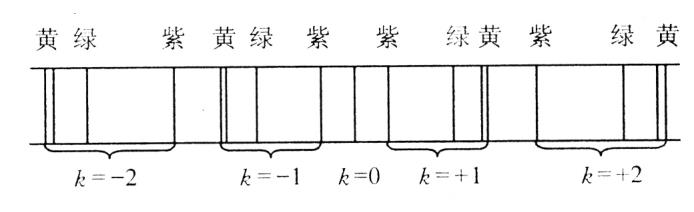
\includegraphics[width=0.92\linewidth]{assets/mercury-spectrum.png}
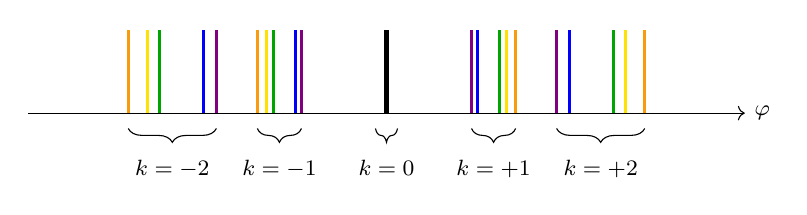
\begin{tikzpicture}[font=\footnotesize, decoration={brace, amplitude=5pt, mirror, raise=1pt}]
  \def\h{1.05}
  \def\yv{1.08}
  \def\yb{1.16}
  \def\yg{1.44}
  \def\yyi{1.52}
  \def\yyii{1.64}
  \draw[->] (-4.55,0) -- (4.55,0);
  \node[right] at (4.55,0) {$\varphi$};
  \draw[line width=2.0pt] (0,0) -- (0,\h);
  \foreach \k in {-2,-1,1,2} {
    \draw[violet, line width=1.05pt] ({\k*\yv},0) -- ({\k*\yv},\h);
    \draw[blue, line width=1.05pt] ({\k*\yb},0) -- ({\k*\yb},\h);
    \draw[green!65!black, line width=1.15pt] ({\k*\yg},0) -- ({\k*\yg},\h);
    \draw[yellow!85!orange, line width=1.1pt] ({\k*\yyi},0) -- ({\k*\yyi},\h);
    \draw[yellow!60!red, line width=1.1pt] ({\k*\yyii},0) -- ({\k*\yyii},\h);
  }
  \draw[decorate] (-2*\yyii,-0.16) -- (-2*\yv,-0.16);
  \node[below=9pt] at (-2*1.36, -0.16) {$k=-2$};
  \draw[decorate] (-\yyii,-0.16) -- (-\yv,-0.16);
  \node[below=9pt] at (-1.36, -0.16) {$k=-1$};
  \draw[decorate] (-0.14,-0.16) -- (0.14,-0.16);
  \node[below=9pt] at (0, -0.16) {$k=0$};
  \draw[decorate] (\yv,-0.16) -- (\yyii,-0.16);
  \node[below=9pt] at (1.36, -0.16) {$k=+1$};
  \draw[decorate] (2*\yv,-0.16) -- (2*\yyii,-0.16);
  \node[below=9pt] at (2*1.36, -0.16) {$k=+2$};
\end{tikzpicture}

  \caption{低压汞灯衍射光谱示意图}
  \label{fig:mercury-spectrum}
\end{figure}

汞灯常见可见谱线中，绿线 $\lambda_{\mathrm{G}}=546.07\,\si{\nano\metre}$，黄双线约为
\[
  \lambda_{\mathrm{Y_I}}=576.96\,\si{\nano\metre},\qquad
  \lambda_{\mathrm{Y_{II}}}=579.07\,\si{\nano\metre}.
\]
若光栅常数已知，精确测定某谱线的衍射角即可求波长；反之，由已知波长可求光栅常数。

\subsection{光栅的角色散和分辨本领}

角色散表征光栅将不同波长分开的能力，定义为单位波长间隔对应的角间距
\begin{equation}
  \label{eq:angular-dispersion-def}
  D=\frac{\mathrm{d}\varphi}{\mathrm{d}\lambda}.
\end{equation}
将光栅方程对 $\lambda$ 微分，得
\begin{equation}
  \label{eq:angular-dispersion}
  D=\frac{k}{d\cos\varphi}.
\end{equation}
由此可见，光栅常数越小、级次越高，角色散越大。对汞灯黄双线，也可用有限差商估计
\begin{equation}
  \label{eq:angular-dispersion-finite}
  D=\frac{\varphi_{\mathrm{Y_{II}}}-\varphi_{\mathrm{Y_I}}}{\lambda_{\mathrm{Y_{II}}}-\lambda_{\mathrm{Y_I}}}.
\end{equation}

分辨本领表征光栅分辨光谱细节的能力。若光栅恰能分开波长为 $\lambda$ 和 $\lambda+\Delta\lambda$ 的两条谱线，则
\begin{equation}
  \label{eq:resolving-power-def}
  R=\frac{\lambda}{\Delta\lambda}.
\end{equation}
根据瑞利判据，一条谱线的光强极大与另一条谱线的极小重合时，两条谱线刚可分辨，由此得到
\begin{equation}
  \label{eq:resolving-power}
  R=kN,
\end{equation}
其中 $N$ 为光栅被照明的总狭缝数。实验中可取黄光 I、II 作为刚被分辨的一对谱线，用 $\lambda=(\lambda_{\mathrm{Y_I}}+\lambda_{\mathrm{Y_{II}}})/2$ 和 $\Delta\lambda=\lambda_{\mathrm{Y_{II}}}-\lambda_{\mathrm{Y_I}}$ 估算实际分辨本领，并与 $kN$ 比较。

\section{实验内容和步骤}

调节分光计前，先熟悉各调节螺钉和锁紧螺钉的位置及作用，如图~\ref{fig:screws} 所示。后续测量必须满足：望远镜能接收平行光；平行光管能发出平行光；望远镜光轴、平行光管光轴均与仪器转轴垂直。

\begin{figure}[htbp]
  \centering
  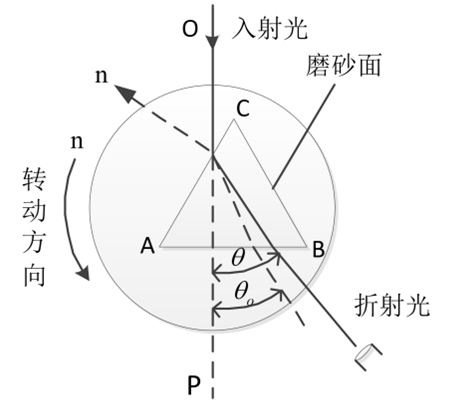
\includegraphics[width=0.36\linewidth]{assets/spectrometer-screws.png}
  \caption{分光计主要调节螺钉}
  \label{fig:screws}
\end{figure}

\subsection{分光计的调节}

\paragraph{目测粗调}
站在仪器前，使目光与望远镜、平行光管和载物台大致处于同一水平。调节望远镜倾斜螺钉、平行光管倾斜螺钉和载物台调平螺钉，使三者大致水平并与转轴垂直。粗调是细调的基础，应反复进行到尽可能好的状态。

\paragraph{调节目镜看清叉丝}
接通望远镜中阿贝目镜的小灯，观察视场下半区是否出现绿色光斑。缓慢调节目镜调焦手轮，直到能清晰看到分划板上的黑叉丝以及绿光区中的绿色亮十字。

\paragraph{自准直法将望远镜调焦到无穷远}
载物台上有三条互成 $120^\circ$ 的标线，分别与台下三个调平螺钉 $a$、$b$、$c$ 对齐。将平面反射镜放在与 $a$ 标线重合、并与 $b$、$c$ 连线垂直的位置，如图~\ref{fig:mirror-placement} 所示。调整载物台高度，使反射镜中心与望远镜光轴大致等高。

\begin{figure}[!htbp]
  \centering
  % 原引用图：assets/mirror-placement.png
  % TikZ 复刻。原图：assets/mirror-placement.png
% 回退：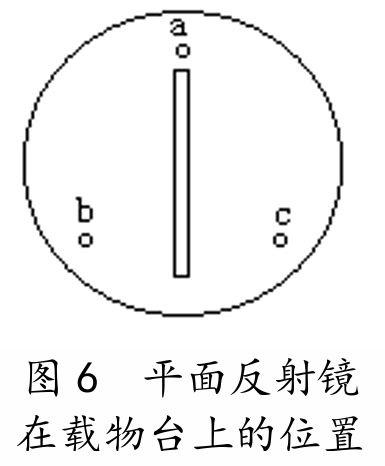
\includegraphics[width=0.32\linewidth]{assets/mirror-placement.png}
\begin{tikzpicture}[font=\small]
  \def\R{2.05}
  \draw[thick] (0,0) circle (\R);
  \foreach \ang in {90,210,330} {
    \draw[thin] (0,0) -- (\ang:\R);
  }
  \filldraw[fill=white, thick] (90:\R) circle (0.16);
  \filldraw[fill=white, thick] (210:\R) circle (0.16);
  \filldraw[fill=white, thick] (330:\R) circle (0.16);
  \node[above=5pt] at (90:\R) {$a$};
  \node[below left] at (210:\R) {$b$};
  \node[below right] at (330:\R) {$c$};
  \filldraw[fill=gray!20, thick] (-0.11,-1.20) rectangle (0.11,1.15);
  \node[right] at (1.15,-0.15) {反射镜};
  \draw[thin] (0.11,0.05) -- (1.05,-0.12);
\end{tikzpicture}

  \caption{平面反射镜在载物台上的位置}
  \label{fig:mirror-placement}
\end{figure}

转动游标盘，使镜面正对望远镜。调节望远镜倾斜螺钉或载物台螺钉 $b$、$c$，直到目镜中出现反射回来的亮斑或模糊亮十字。松开目镜套筒锁紧螺钉，前后移动套筒，使亮十字最清晰并与叉丝无视差，再锁紧套筒。此时望远镜已适合接收平行光。若在目镜中找不到反射像，可先在望远镜外侧用眼睛寻找反射亮点，再把眼睛高度和载物台倾斜调到与目镜中心等高。

\paragraph{各半调节法使望远镜光轴垂直于仪器转轴}
先调节载物台螺钉，使亮十字落在分划板上叉丝的上交叉点附近，说明镜面已大致垂直于望远镜光轴。将载物台连同平面镜转过 $180^\circ$。若两准线不再重合，先调节螺钉 $b$ 或 $c$，使亮十字与上叉丝的间距缩小一半，再调节望远镜倾斜螺钉使二者重合，如图~\ref{fig:half-adjust} 所示。再转 $180^\circ$ 检查。反复进行，直到平面镜的两个面反射回来的亮十字都落在上交叉点上。此时望远镜光轴已垂直于分光计转轴。

\begin{figure}[!htbp]
  \centering
  % 原引用图：assets/half-adjust.png
  % TikZ 复刻。原图：assets/half-adjust.png
% 回退：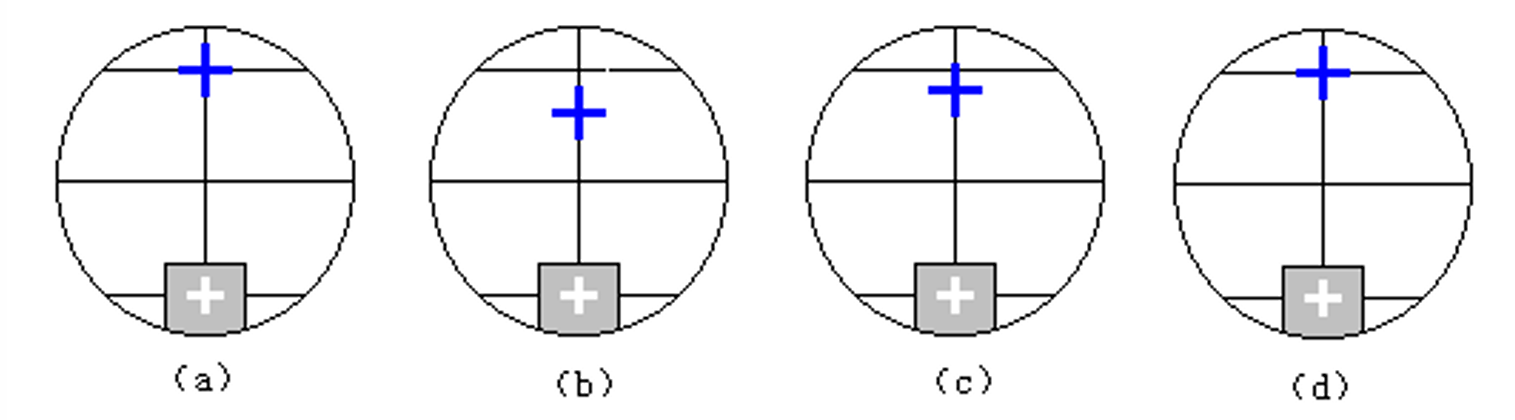
\includegraphics[width=\linewidth]{assets/half-adjust.png}
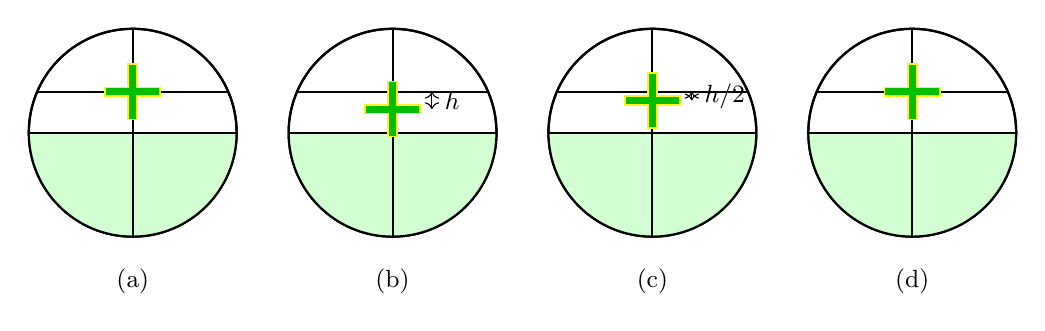
\begin{tikzpicture}[font=\small]
  \def\R{1.32}
  \foreach \xshift/\gy/\lab/\shownote/\notetext in {
      0/0.52/{(a)}/0/{},
      3.3/0.30/{(b)}/1/{$h$},
      6.6/0.41/{(c)}/1/{$h/2$},
      9.9/0.52/{(d)}/0/{}
    } {
    \begin{scope}[shift={(\xshift,0)}]
      \draw[thick] (0,0) circle (\R);
      \begin{scope}
        \clip (0,0) circle (\R);
        \fill[green!18] (-\R-0.1,-\R-0.1) rectangle (\R+0.1,0);
        \draw[line width=0.7pt] (0,-\R) -- (0,\R);
        \draw[line width=0.7pt] (-\R,0) -- (\R,0);
        \draw[line width=0.7pt] (-\R,0.52) -- (\R,0.52);
        \draw[line width=3.8pt, yellow!90] (-0.36,\gy) -- (0.36,\gy);
        \draw[line width=3.8pt, yellow!90] (0,\gy-0.36) -- (0,\gy+0.36);
        \draw[line width=2.5pt, green!75!black] (-0.34,\gy) -- (0.34,\gy);
        \draw[line width=2.5pt, green!75!black] (0,\gy-0.34) -- (0,\gy+0.34);
      \end{scope}
      \draw[thick] (0,0) circle (\R);
      \ifnum\shownote=1
        \draw[<->] (0.50,0.52) -- (0.50,\gy);
        \node[right] at (0.54,{0.5*(0.52+\gy)}) {\notetext};
      \fi
      \node[below] at (0,-\R-0.28) {\lab};
    \end{scope}
  }
\end{tikzpicture}

  \caption{各半调节法：目镜中看到的亮十字与叉丝}
  \label{fig:half-adjust}
\end{figure}

若转过 $180^\circ$ 后完全看不到另一面的反射像，先回到能看到亮十字的一面，把亮十字调到上交叉点下方，再调载物台螺钉使其回到上交叉点，然后继续对各面作各半调节。

\paragraph{调节载物台法线平行于转轴}
望远镜倾斜螺钉以及载物台 $b$、$c$ 螺钉此后不再改动。将平面镜改放到与 $a$ 标线垂直、与 $b$、$c$ 连线平行的位置，只调节螺钉 $a$，使反射亮十字仍落在上交叉点。这样载物台平面即与望远镜光轴扫过的平面平行。

\paragraph{调节平行光管}
开启汞灯照亮狭缝，把已调好的望远镜转到正对平行光管。松开狭缝套筒螺钉，前后移动狭缝，直到狭缝像细锐清晰并与叉丝无视差，此时平行光管已发出平行光。狭缝宽度宜调到与叉丝线宽相近，约 $1\,\si{\milli\metre}$。再调节平行光管倾斜螺钉，使狭缝像被分划板中央水平叉丝平分，从而使平行光管光轴也垂直于仪器转轴。最后将叉丝竖线对准狭缝像中央并固定望远镜，作为入射光方位的参考。

\subsection{光栅的调节}

用光栅方程~\eqref{eq:grating-equation} 测量时必须满足：入射平行光垂直于光栅表面；零级两侧谱线等高。望远镜已经调好后，不得再动其倾斜螺钉。

\begin{enumerate}[label=\arabic*)]
  \item 把光栅直立在载物台中部，使光栅平面垂直平分调平螺钉 1、2 的连线，螺钉 3 位于光栅平面内，如图~\ref{fig:grating-placement} 所示。
  \item 先让望远镜对准平行光管，使狭缝像与竖叉丝重合并固定望远镜。转动载物台，以光栅面为反射面，用自准直法只调节螺钉 1、2，使反射回来的绿色亮十字与分划板上叉丝上交叉点重合，如图~\ref{fig:crosshair} 所示。此时光栅平面垂直于平行光管光轴，并与仪器转轴平行，随即固定游标盘。光栅不必再转 $180^\circ$。
  \item 透射光栅常同时出现一强一弱两个十字反射像。强像来自前表面，弱像来自后表面。调整时只以强像为基准，忽略弱像。
  \item 松开望远镜，观察正、负一级谱线。若叉丝交点不在各谱线中央，只调节螺钉 3，使两侧谱线等高，如图~\ref{fig:spectral-height} 所示。反复检查垂直入射与两侧等高，直到同时满足。
\end{enumerate}

\begin{figure}[htbp]
  \centering
  % 原引用图：assets/grating-placement.png
  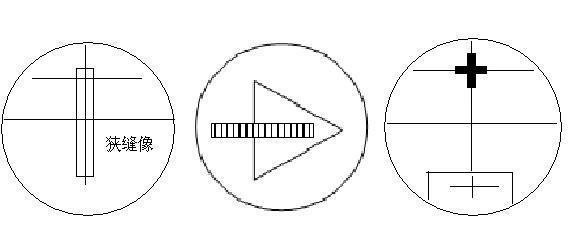
\includegraphics[width=0.70\linewidth]{assets/grating-placement.png}
  \caption{光栅在载物台上的位置}
  \label{fig:grating-placement}
\end{figure}

\begin{figure}[htbp]
  \centering
  \begin{minipage}[t]{0.42\linewidth}
    \centering
    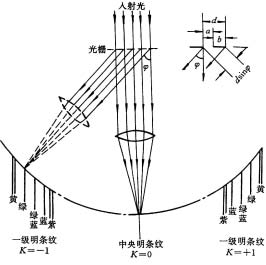
\includegraphics[width=0.72\linewidth]{assets/crosshair.png}
    \caption{光栅自准直调节}
    \label{fig:crosshair}
  \end{minipage}
  \hfill
  \begin{minipage}[t]{0.52\linewidth}
    \centering
    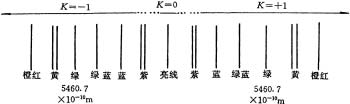
\includegraphics[width=\linewidth]{assets/spectral-height.png}
    \caption{调节零级两侧谱线等高}
    \label{fig:spectral-height}
  \end{minipage}
\end{figure}

\subsection{用平面衍射光栅测量谱线波长和光栅常数}

分光计按要求调好后，必须固定载物台和游标盘，只让望远镜绕主轴转动。测量前先左右转动望远镜，确认 $k=\pm1$ 和 $k=\pm2$ 的谱线清晰可见，且同级谱线相对零级的偏角大致相等，以此检验光栅是否垂直于入射光。读数时应单方向转动望远镜，避免空程差；每一位置同时记录左、右窗口。

\begin{enumerate}[label=\arabic*)]
  \item 已知光栅常数 $d=0.01\,\si{\milli\metre}$（$N=100\,\mathrm{mm}^{-1}$）时，测量汞绿光 $k=\pm1$、$k=\pm2$ 谱线位置，由式~\eqref{eq:diffraction-angle} 和式~\eqref{eq:grating-equation} 计算波长。
  \item 换上待测光栅。已知汞绿光 $\lambda=546.07\,\si{\nano\metre}$，分别测量其 $k=\pm1$、$k=\pm2$ 谱线位置，求待测光栅的 $d$ 和 $N$。
  \item 仍用该待测光栅，测量黄光 I、黄光 II 的 $k=\pm1$ 谱线位置，求黄双线波长。
  \item 由式~\eqref{eq:angular-dispersion} 计算角色散 $D$，并由式~\eqref{eq:resolving-power-def}、式~\eqref{eq:resolving-power} 讨论分辨本领。
\end{enumerate}

开始正式读数前，应先移动目镜观察一周，确认二级谱线中两条黄线仍可分辨后再测量。

\begin{LabRecordTable}
  \centering
  \caption{已知光栅测绿光波长（$d=0.01\,\si{\milli\metre}$）}
  \label{table:green}
  \renewcommand{\arraystretch}{1.05}
  \setlength{\tabcolsep}{3pt}
  \footnotesize
  \begin{tabularx}{\textwidth}{C{1.5cm} *{4}{Y} Y}
    \toprule
    \multirow{2}{*}[-0.6ex]{级次} & \multicolumn{2}{c}{右侧} & \multicolumn{2}{c}{左侧} & \multirow{2}{*}[-0.6ex]{$\varphi$} \\
    \cmidrule(lr){2-3}\cmidrule(lr){4-5}
    & 左窗 & 右窗 & 左窗 & 右窗 & \\
    \midrule
    $k=\pm1$ & $336^\circ30'$ & $156^\circ30'$ & $342^\circ45'$ & $162^\circ45'$ & $3.125^\circ$ \\
    $k=\pm2$ & $328^\circ50'$ & $148^\circ50'$ & $341^\circ30'$ & $161^\circ30'$ & $6.333^\circ$ \\
    \bottomrule
  \end{tabularx}
\end{LabRecordTable}

\begin{LabRecordTable}
  \centering
  \caption{已知绿光波长测待测光栅常数（$\lambda=546.07\,\si{\nano\metre}$）}
  \label{table:unknown-grating}
  \renewcommand{\arraystretch}{1.05}
  \setlength{\tabcolsep}{3pt}
  \footnotesize
  \begin{tabularx}{\textwidth}{C{1.5cm} *{4}{Y} Y}
    \toprule
    \multirow{2}{*}[-0.6ex]{级次} & \multicolumn{2}{c}{右侧} & \multicolumn{2}{c}{左侧} & \multirow{2}{*}[-0.6ex]{$\varphi$} \\
    \cmidrule(lr){2-3}\cmidrule(lr){4-5}
    & 左窗 & 右窗 & 左窗 & 右窗 & \\
    \midrule
    $k=\pm1$ & $328^\circ55'$ & $148^\circ55'$ & $347^\circ45'$ & $167^\circ45'$ & $9.417^\circ$ \\
    $k=\pm2$ & $357^\circ30'$ & $177^\circ30'$ & $319^\circ10'$ & $139^\circ10'$ & $19.167^\circ$ \\
    \bottomrule
  \end{tabularx}
\end{LabRecordTable}

\begin{LabRecordTable}
  \centering
  \caption{待测光栅测黄光 I、II 波长}
  \label{table:yellow}
  \renewcommand{\arraystretch}{1.05}
  \setlength{\tabcolsep}{2pt}
  \footnotesize
  \begin{tabularx}{\textwidth}{C{1.5cm} C{1.5cm} *{4}{Y} Y}
    \toprule
    \multirow{2}{*}[-0.6ex]{谱线} & \multirow{2}{*}[-0.6ex]{级次} & \multicolumn{2}{c}{右侧} & \multicolumn{2}{c}{左侧} & \multirow{2}{*}[-0.6ex]{$\varphi$} \\
    \cmidrule(lr){3-4}\cmidrule(lr){5-6}
    & & 左窗 & 右窗 & 左窗 & 右窗 & \\
    \midrule
    黄光 I & $k=\pm1$ & $328^\circ30'$ & $148^\circ30'$ & $348^\circ20'$ & $168^\circ20'$ & $9.917^\circ$ \\
    黄光 II & $k=\pm1$ & $358^\circ30'$ & $178^\circ30'$ & $338^\circ30'$ & $158^\circ30'$ & $10.000^\circ$ \\
    \bottomrule
  \end{tabularx}
\end{LabRecordTable}

\section{数据处理}

表~\ref{table:green}--表~\ref{table:yellow} 均为单次测量。表中 $\varphi$ 一律由左右窗口读数按式~\eqref{eq:diffraction-angle} 计算，不采用记录表上的手算值。波长和光栅常数分别由
\begin{equation}
  \label{eq:lambda-from-d}
  \lambda=\frac{d\sin\varphi}{\lvert k\rvert}
\end{equation}
和
\begin{equation}
  \label{eq:d-from-lambda}
  d=\frac{\lvert k\rvert\lambda}{\sin\varphi},\qquad N=\frac{1}{d}
\end{equation}
给出。分光计最小分度为 $1'$，按均匀分布取
\[
  u_\theta=\frac{1'}{\sqrt{3}}=0.00962^\circ.
\]
四个游标独立时
\begin{equation}
  \label{eq:phi-uncertainty}
  u_\varphi=\frac{1}{2}u_\theta=0.00481^\circ,
\end{equation}
相对不确定度由 $u_\varphi\cot\varphi$ 传递（$\varphi$ 化为弧度）。

\subsection{已知光栅测绿光波长}

已知 $d=0.01\,\si{\milli\metre}$。由表~\ref{table:green}，
\begin{align*}
  k=\pm1,\ \varphi=3.125^\circ:\quad
  \lambda_1
  &=545.15\,\si{\nano\metre},\\
  k=\pm2,\ \varphi=6.333^\circ:\quad
  \lambda_2
  &=551.56\,\si{\nano\metre}.
\end{align*}
平均 $\bar\lambda_{\mathrm{G}}=548.35\,\si{\nano\metre}$。相对汞绿线 $546.07\,\si{\nano\metre}$，两级相对误差为 $-0.17\%$ 和 $+1.01\%$，平均 $+0.42\%$。相应的 $u_{\lambda_1}=0.84\,\si{\nano\metre}$，$u_{\lambda_2}=0.42\,\si{\nano\metre}$。

\subsection{已知绿光波长测待测光栅常数}

以 $\lambda=546.07\,\si{\nano\metre}$ 和表~\ref{table:unknown-grating} 代入式~\eqref{eq:d-from-lambda}，
\begin{align*}
  k=\pm1,\ \varphi=9.417^\circ:\quad
  d_1&=3.338\times10^{-3}\,\si{\milli\metre},
  \quad N_1=299.6\,\mathrm{mm}^{-1},\\
  k=\pm2,\ \varphi=19.167^\circ:\quad
  d_2&=3.326\times10^{-3}\,\si{\milli\metre},
  \quad N_2=300.6\,\mathrm{mm}^{-1}.
\end{align*}
平均
\[
  \bar d=3.332\times10^{-3}\,\si{\milli\metre},\qquad
  \bar N=300.1\,\mathrm{mm}^{-1}.
\]
两级相差约 $0.3\%$，待测光栅可定为 $300\,\mathrm{mm}^{-1}$。$u_d/d$ 在一级为 $0.051\%$，二级为 $0.024\%$。

\subsection{待测光栅测黄光波长}

黄光在换上待测光栅后测量，两条都取 $k=\pm1$。记录时 I、II 可能对调，这里按衍射角从小到大指定：$\varphi=9.917^\circ$ 为黄光 I，$10.000^\circ$ 为黄光 II。用 $\bar d$ 代入式~\eqref{eq:lambda-from-d}，
\begin{align*}
  \lambda_{\mathrm{Y_I}}
  &=\bar d\sin 9.917^\circ\times10^{6}
  =573.8\,\si{\nano\metre},\\
  \lambda_{\mathrm{Y_{II}}}
  &=\bar d\sin 10.000^\circ\times10^{6}
  =578.6\,\si{\nano\metre}.
\end{align*}
相对 $576.96$、$579.07\,\si{\nano\metre}$，误差为 $-0.54\%$ 和 $-0.08\%$。$u_\lambda$ 约为 $0.28\,\si{\nano\metre}$。角色散按式~\eqref{eq:angular-dispersion} 计算。

\subsection{角色散和分辨本领}

由式~\eqref{eq:angular-dispersion}，已知光栅在绿光处
\[
  D_1=\frac{1}{d\cos 3.125^\circ}=0.344'/\si{\nano\metre},\qquad
  D_2=\frac{2}{d\cos 6.333^\circ}=0.692'/\si{\nano\metre}.
\]
待测光栅在绿光处
\[
  D_1'=\frac{1}{\bar d\cos 9.417^\circ}=1.046'/\si{\nano\metre},\qquad
  D_2'=\frac{2}{\bar d\cos 19.167^\circ}=2.185'/\si{\nano\metre}.
\]
在黄双线附近（$k=1$）
\[
  D_{\mathrm{Y}}=\frac{1}{\bar d\cos 10.06^\circ}=1.048'/\si{\nano\metre}.
\]
光栅越密、级次越高，角色散越大。

黄双线取 $\lambda=578.02\,\si{\nano\metre}$、$\Delta\lambda=2.11\,\si{\nano\metre}$，刚可分辨时
\[
  R=\frac{\lambda}{\Delta\lambda}=274.
\]
理论值 $R=kN$。平行光管照明宽度按约 $20\,\si{\milli\metre}$ 估计，则已知光栅 $N\approx2.0\times10^{3}$，待测光栅 $N\approx6.0\times10^{3}$。$k=1$ 时理论分辨本领已大于 274，与实验中仍能分开黄双线相符。

\subsection{结论和误差}

用 $100\,\mathrm{mm}^{-1}$ 光栅测得汞绿线平均波长 $548.35\,\si{\nano\metre}$，相对误差 $0.42\%$。用汞绿线测得待测光栅 $\bar N=300.1\,\mathrm{mm}^{-1}$，两级一致。黄双线是在该 $300\,\mathrm{mm}^{-1}$ 光栅上、以 $k=\pm1$ 测的，得到 $573.8$、$578.6\,\si{\nano\metre}$，相对误差均小于 $1\%$。

主要误差还有叉丝对准、空程以及单次测量没有 A 类分量。B 类按 $1'$ 估计。

% 本次教师说明不做思考题。
\iffalse
\section{思考题}

\begin{enumerate}[label=\arabic*. ]
  \item 分光计调整的要求是什么？如何实现？

  需要同时满足五条：望远镜聚焦于无穷远，能接收平行光；望远镜光轴垂直于仪器转轴；载物台法线平行于转轴；平行光管发出平行光；平行光管光轴也垂直于转轴。实现方法是：先目测粗调，再用自准直法把望远镜调焦到无穷远；用平面镜转 $180^\circ$ 配合各半调节，使两面反射的亮十字都落在分划板上叉丝上交叉点；改放平面镜方位后只调第三个螺钉，使载物台水平；最后用已调好的望远镜观察狭缝像，伸缩狭缝套筒至无视差，并调节平行光管倾斜，使狭缝像被中央水平叉丝平分。

  \item 调节分光计时，若反射像不清晰，能否再调目镜视度手轮使反射像清晰？若狭缝像不清晰，能否再调目镜或把望远镜套筒拉出、推进？若狭缝像偏高或偏低，能否再调望远镜倾斜螺钉？

  都不能。目镜调好后，分划板已经成像在明视距离处，反射像不清晰应前后移动目镜套筒，改变物镜与分划板的距离。望远镜焦距调好后不能再动，狭缝像不清晰应伸缩平行光管的狭缝套筒。望远镜光轴已经垂直于转轴，狭缝像高低应由平行光管的倾斜螺钉来纠正。

  \item 光栅光谱与棱镜光谱有哪些不同之处？

  光栅光谱来自衍射和多光束干涉，服从光栅方程，谱线以零级为中心左右对称，同级按短波到长波排列，衍射角与波长近于线性关系，角色散由 $d$ 和 $k$ 决定，分辨本领为 $kN$。棱镜光谱来自折射，依赖材料色散，谱线只出现在棱镜一侧，无对称零级，偏向角与波长非线性，短波偏折更显著。光栅光谱还可能出现缺级，棱镜光谱没有这一现象。

  \item 实验时并不要求仪器转轴过光栅面，这对测量衍射角有无影响？

  没有实质影响。衍射角是衍射光相对光栅法线的夹角，不是谱线的绝对方位角。实验用左右同级谱线方位角之差的一半来求 $\varphi$，转轴偏心只改变绝对读数，不改变两侧相对零级的对称关系。只要光栅平面已垂直于平行光管光轴、刻痕平行于转轴，光谱对称，转轴是否穿过光栅面就不进入 $\varphi$ 的计算结果。

  \item 用自准直法调整光栅方位时，往往同时看到一强一弱两个十字反射像。它们是怎样形成的？应如何处理？

  强像由光栅前表面（空气--玻璃界面）反射形成，光强损失小；弱像由后表面反射形成，光线往返穿过玻璃基底，因而较暗。调整时只以强像为准，调节载物台螺钉 1、2，使强像与上叉丝重合，忽略弱像，并且不再改动已经调好的望远镜。

  \item 如果光栅位置不正确，或平行光管狭缝过宽、过窄，对测量有什么影响？

  光栅平面若不正交于入射光，左右同级衍射角不再相等，由式~\eqref{eq:grating-equation} 算出的 $\lambda$ 或 $d$ 会系统偏离；刻痕若与转轴不平行，两侧谱线不等高，叉丝难以对准谱线中心。狭缝过宽会使谱线加宽、黄双线重叠，降低分辨本领；过窄则光强弱，高级次谱线难以辨认。实验中把缝宽调到约 $1\,\si{\milli\metre}$，兼顾清晰度和亮度。

  \item 本实验采取了哪些措施提高测量准确度？

  主要措施有：用自准直和各半调节把分光计调到测量状态；光栅调节时不再改动望远镜倾斜；左右窗口同时读数以消除偏心差；用左右同级谱线求衍射角以减弱不对称和转轴位置的影响；单方向转动望远镜以减小空程；对绿光和待测光栅同时测量 $k=\pm1$ 与 $k=\pm2$ 以便互校；测量前先确认二级黄双线仍可分辨，并检查同级左右偏角是否近似相等。
\end{enumerate}
\fi

\insertSignedDataPage

\end{document}
